\chapter{Monte Carlo Solution Methods for Linear Systems}
\label{ch:stochastic_methods}
An alternative approach to approximate matrix inversion is to employ
Monte Carlo methods that sample a distribution with an expectation
value equivalent to that of the inverted operator. Such methods have
been in existence for decades with the earliest reference noted here
an enjoyable manuscript published in 1950 by Forsythe and Leibler
\citep{forsythe_matrix_1950}. In their outline, Forsythe and Liebler
in fact credit the creation of this technique to J. Von Neumann and
S.M. Ulam some years earlier than its publication. In 1952 Wasow
provided a more formal explanation of Von Neumann and Ulam's method
\citep{wasow_note_1952} and Hammersley and Handscomb's 1964 monograph
\citep{hammersley_monte_1964} and Spanier and Gelbard's 1969 book
\citep{spanier_monte_1969} present additional detail on this topic
using a collection of references from the 1950's and early 1960's.

%%---------------------------------------------------------------------------%%
\section{Preliminaries}
\label{sec:mc_preliminaries}
We begin our discussion of Monte Carlo methods using these texts by
seeking a solution to Eq~(\ref{eq:linear_problem}). For a given linear
operator $\ve{A}$, we can use diagonal splitting in a similar manner
as the stationary method in Eq~(\ref{eq:linear_split_equation2}) to
define the following operator\footnote{It should be noted that
  non-diagonal splittings have been recently explored in
  \citep{srinivasan_monte_2010} and have the potential to improve
  efficiency.}:
\begin{equation}
  \ve{H} = \ve{I} - \ve{A}\:,
  \label{eq:linear_mc_iteration_matrix}
\end{equation}
such that we are solving the system:
\begin{equation}
  \ve{x} = \ve{H} \ve{x} + \ve{b}\:.
  \label{eq:richardson_split}
\end{equation}
We can then form an alternative representation for $\ve{A}^{-1}$ by
generating the \textit{Neumann series}:
\begin{equation}
  \ve{A}^{-1} = (\ve{I}-\ve{H})^{-1} = \sum_{k=0}^{\infty} \ve{H}^k\:,
  \label{eq:neumann_series}
\end{equation}
which will converge if the spectral radius of $\ve{H}$ is less than
1. If we then apply this Neumann series to the right hand side of
Eq~(\ref{eq:linear_problem}) we acquire the solution to the linear
problem:
\begin{equation}
  \ve{A}^{-1}\ve{b} = \sum_{k=0}^{\infty} \ve{H}^k\ve{b} = \ve{x}\:.
  \label{eq:neumann_solution}
\end{equation}
An approximation of this summation by truncation will therefore lead
to an approximation of the solution. If we expand the summation with a
succession of matrix-vector multiply operations, we arrive at an
alternative perspective of this summation by considering its $i^{th}$
component:
\begin{equation}
  x_i = \sum_{k=0}^{\infty}\sum_{i_1}^{N}\sum_{i_2}^{N}\ldots
  \sum_{i_k}^{N}h_{i,i_1}h_{i_1,i_2}\ldots h_{i_{k-1},i_k}b_{i_k}\:,
  \label{eq:expanded_neumann_solution}
\end{equation}
which can interpreted as a series of transitions between states,
\begin{equation}
 \nu = i \rightarrow i_1 \rightarrow \cdots \rightarrow i_{k-1}
 \rightarrow i_{k}\:,
  \label{eq:mc_walk_permutation}
\end{equation}
in $\ve{H}$ where $\nu$ is interpreted as a particular random walk
sequence permutation. We can generate these sequences of transitions
through Monte Carlo random walks by assigning them both a probability
and weight. As a reinterpretation of the iteration matrix, we then
form the \textit{Neumann-Ulam decomposition} of \ve{H}:
\begin{equation}
  \ve{H} = \ve{P} \circ \ve{W}\:,
  \label{eq:neumann_ulam_decomposition}
\end{equation}
where $\circ$ denotes the Hadamard product operation\footnote{The
  Hadamard product $\ve{A} = \ve{B} \circ \ve{C}$ is defined
  element-wise as $a_{ij} = b_{ij} c_{ij}$.}, $\ve{P}$ denotes the
transition probability matrix, and $\ve{W}$ denotes the transition
weight matrix. This decomposition, a generalization of Dimov's work
\citep{dimov_new_1998}, is an extension of the original Neumann-Ulam
scheme in that now a weight cutoff can be used to terminate a random
walk sequence and therefore truncate the Neumann series it is
approximating. The formulation of $\ve{P}$ and $\ve{W}$ will be
dependent on whether we choose a direct or adjoint Monte Carlo
sequence to estimate the state transitions in
Eq~(\ref{eq:expanded_neumann_solution}).

%%---------------------------------------------------------------------------%%
\section{Direct Method}
\label{sec:direct_mc}
In the context of matrix inversion, a direct method resembles an
adjoint Monte Carlo method in the reactor physics community where the
solution state is sampled and the source terms that contribute to it
are assembled. To achieve this, we build the direct method
Neumann-Ulam decomposition per Dimov's approach by first choosing a
probability matrix that is a row scaling of $\ve{H}$ such that its
components are:
\begin{equation}
  p_{ij} = \frac{|h_{ij}|}{\sum_j |h_{ij}|}\:.
  \label{eq:direct_probability}
\end{equation}
From this, we then see that the probability of transitioning from a
state $i$ to a state $j$ is implicitly linked to the original operator
$\ve{A}$ in that those terms with large values, and therefore those
that make the greatest contribution to the numerical solution, will be
sampled with a higher probability than smaller terms. In addition, the
row scaling provides a normalization over the state to which we are
transitioning such that $\sum_j p_{ij} = 1$, meaning that we sample
the probabilities over the rows of the matrix. The components of
the weight matrix are then defined by
Eq~(\ref{eq:neumann_ulam_decomposition}) as:
\begin{equation}
  w_{ij} = \frac{h_{ij}}{p_{ij}}\:.
  \label{eq:direct_weight}
\end{equation}
It should be noted here that if $\ve{A}$ is sparse, then $\ve{H}$,
$\ve{P}$, and $\ve{W}$ must be sparse as well by
definition. Additionally, we only compute $\ve{P}$ and $\ve{W}$ from
the non-zero elements of $\ve{H}$ as those components that are zero
will not participate in the random walk. Doing so prevents an
infinite weight from being generated in Eq~(\ref{eq:direct_weight})
and eliminates unnecessary computations.

Using these matrices, we can then form the expectation value of the
direct solution. For a given random walk permutation $\nu$ with $k$
events, we define the weight of that permutation to be:
\begin{equation}
  W_{m} = w_{i,i_1} w_{i_1,i_2} \cdots w_{i_{m-1},i_m}\:,
  \label{eq:direct_permutation_weight}
\end{equation}
such that the weight of each transition event contributes to the
total. The contribution to the solution from a particular random walk
permutation is then:
\begin{equation}
  X_{\nu}(i_0 = i) = \sum_{m=0}^k W_{m} b_{i_m}\:,
  \label{eq:direct_permutation_contribution}
\end{equation}
where $X_{\nu}(i_0 = i)$ signifies that the solution state in which we
are tallying defines state $i$.  We can interpret this precisely as
before in that during the random walk we collect the source in the
states that are visited and apply them to the solution tally. We then
define the probability that a particular random walk permutation of
$k$ events will occur:
\begin{equation}
  P_{\nu} = p_{i,i_1} p_{i_1,i_2} \cdots p_{i_{k-1},i_k}\:.
  \label{eq:direct_permutation_probability}
\end{equation}
Finally, we define the expectation value of $X$ to be the collection
of all random walk permutations and their probabilities:
\begin{equation}
  E\{X(i_0 = i)\} = \sum_{\nu} P_{\nu} X_{\nu}\:,
  \label{eq:direct_expectation_value}
\end{equation}
which, if expanded, directly recovers the exact solution:
\begin{equation}
  \begin{split}
    E\{X(i_0 = i)\}
    &=\sum_{k=0}^{\infty}\sum_{i_1}^{N}\sum_{i_2}^{N}\ldots
    \sum_{i_k}^{N} p_{i,i_1}p_{i_1,i_2}\ldots p_{i_{k-1},i_k}
    w_{i,i_1}w_{i_1,i_2}\ldots w_{i_{k-1},i_k} b_{i_k}\\ &= x_i\:,
  \end{split}
  \label{eq:direct_expectation_expansion}
\end{equation}
therefore providing an unbiased Monte Carlo estimator. 

In cases where we seek only approximate solutions, we need only to
perform a minimal number of random walks in order to generate an
approximation for $\ve{x}$. If we are only to approximate the
solution, we also need conditions by which we may terminate a random
walk. We do this by noticing that the factors added to
Eq~(\ref{eq:direct_permutation_weight}) will become diminishingly
small due to their definition in Eq~(\ref{eq:direct_weight}) and
therefore their contributions to the solution estimate will become
negligible. Using this, we choose terminate a random walk sequence
with a \textit{weight cutoff}, $W_c$, that is enforced when $W_m <
W_c$ for a particular random walk permutation.

\subsection{Direct Method: Evolution of a Solution}
\label{subsec:direct_evolution}

As a means of visually demonstrating the direct Monte Carlo method,
consider a 2-dimensional thermal diffusion problem with sources on the
left and right hand sides of the domain and a smaller uniform source
as shown in Figure~\ref{fig:heat_setup}.
\begin{figure}[h!]
  \begin{center}
    \scalebox{1.0}{ \input{chapters/mc_background/heat_eq_setup.pdftex_t} }
  \end{center}
  \caption{\textbf{Problem setup for 2D heat equation.}
    \textit{Dirichlet conditions are set for the temperature on all 4
      boundaries of the Cartesian grid. Background source of 1/5 the
      value of the boundary sources present. $50 \times 50$ grid.}}
  \label{fig:heat_setup}
\end{figure}
For this problem, the number of histories used to compute the solution
at each state in the domain was increased from 1 to 1000 in order to
show its effects on the solution and the statistical nature of the
method. Figure~\ref{fig:direct_evolution} gives these results.
\begin{figure}[h!]
  \begin{center}
    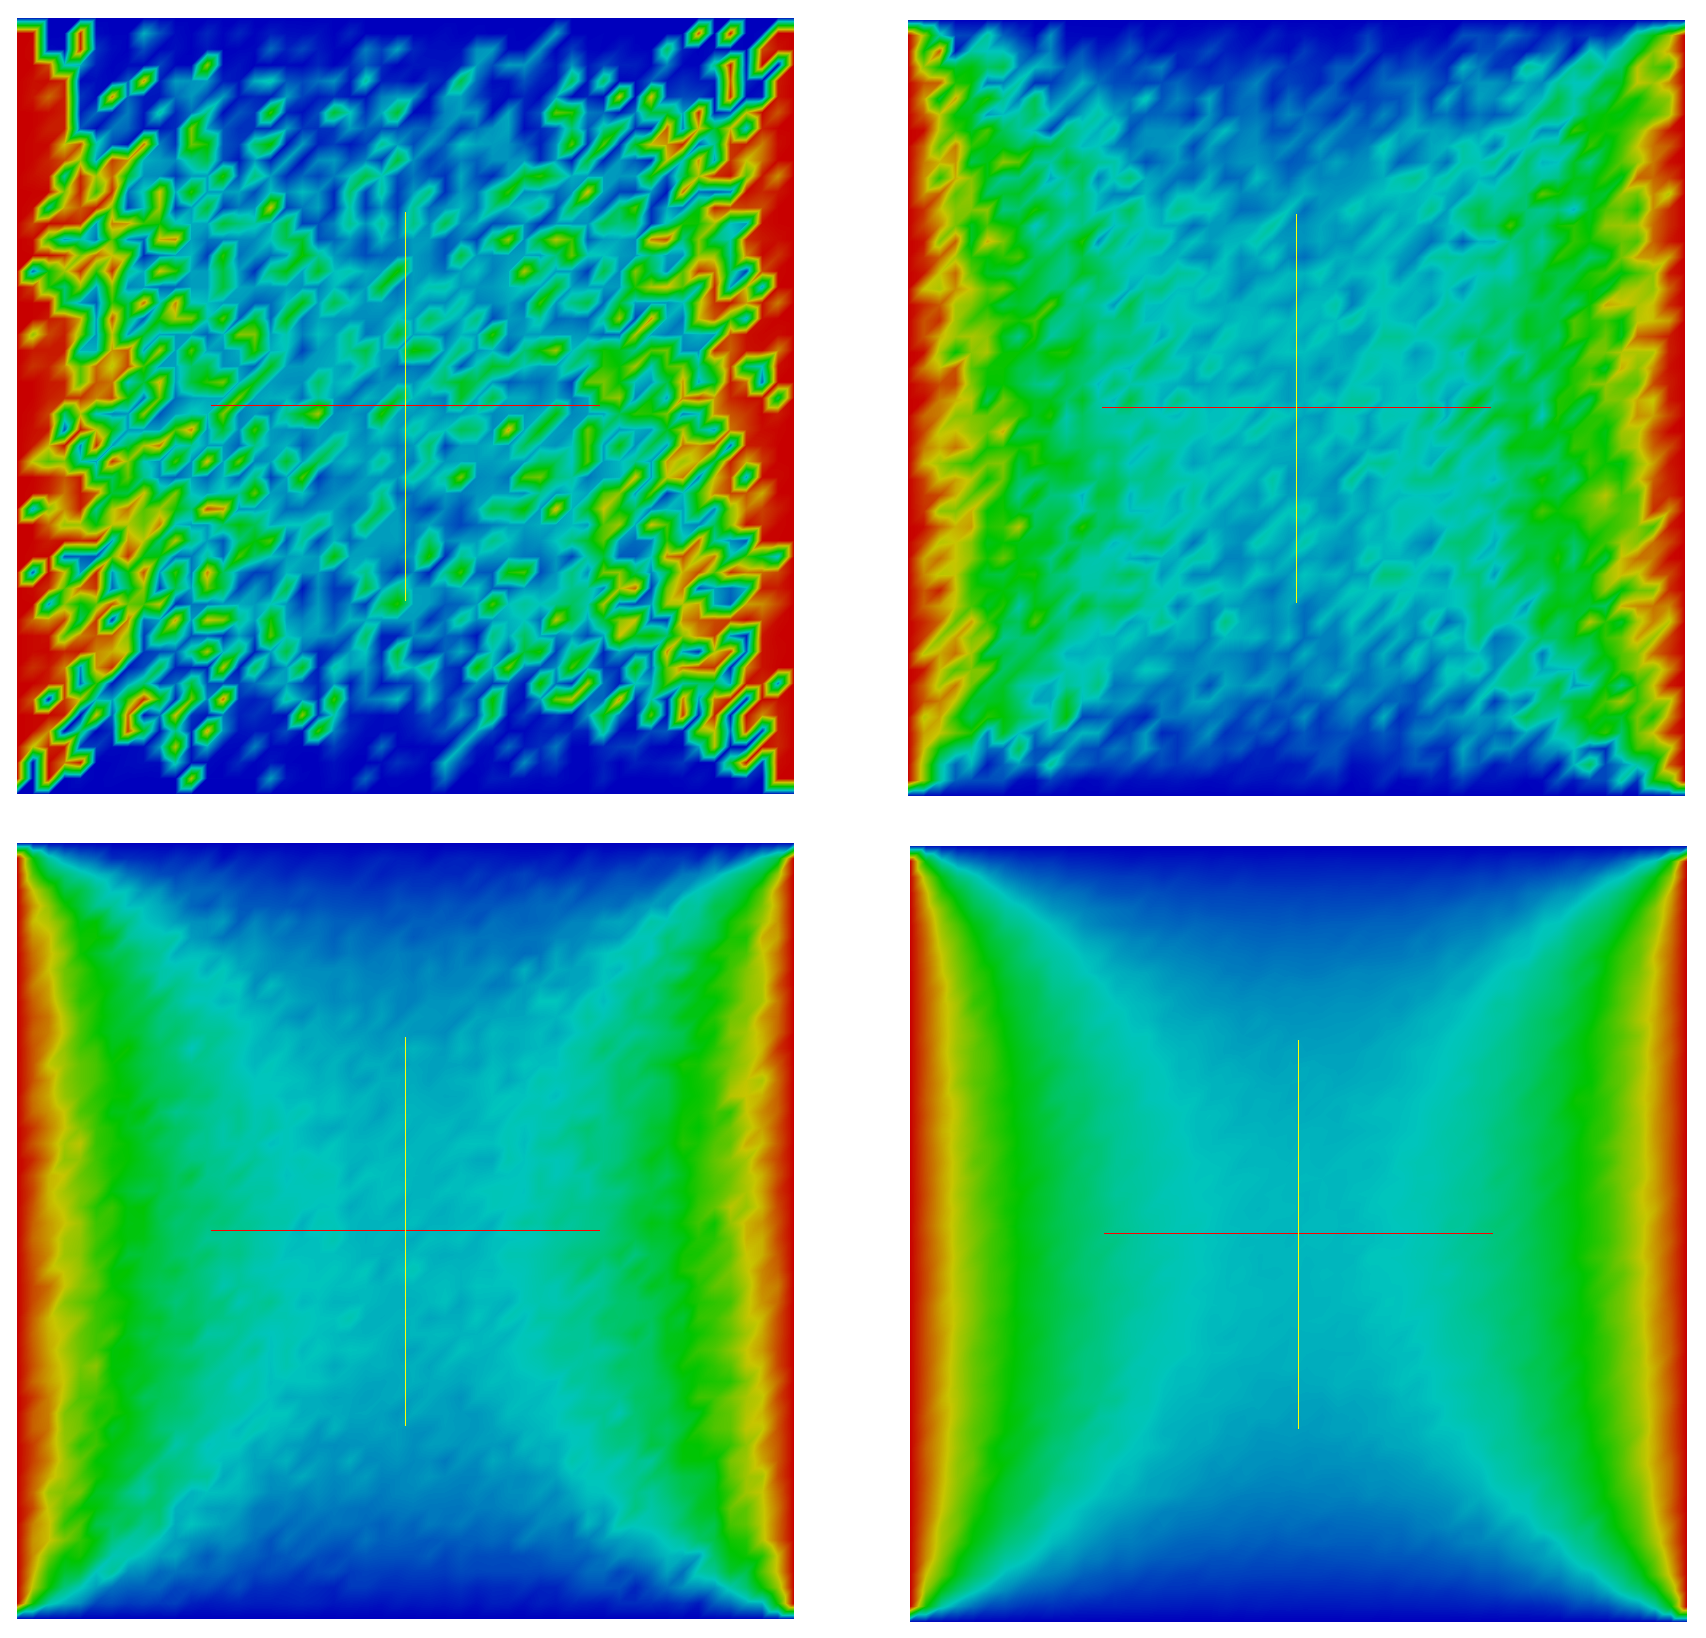
\includegraphics[width=5in]{chapters/mc_background/direct_evolution.png}
  \end{center}
  \caption{\textbf{Direct Monte Carlo solution to the heat equation
      with varying numbers of histories.} \textit{Top left: 1 history
      per state. Top right: 10 histories per state. Bottom left: 100
      histories per state. Bottom right: 1000 histories per state.}}
  \label{fig:direct_evolution}
\end{figure}
As the number of histories used per state is increased, the
statistical variance of the solutions is decreased as more tallies are
made. At 1000 histories per state, enough tallies have been made to
generate a reasonable estimate for the structure of the solution.

\subsection{Estimator Variance}
\label{subsec:estimator_variance}
We can compute the variance of the estimator through traditional
methods by defining the variance, $\sigma_i$, for each component in
the solution:
\begin{equation}
  {\sigma_i}^2 = E\{X(i_0 = i) - (\ve{A}^{-1}\ve{b})_i\}^2 = E\{X(i_0
  = i)^2\} - x_i^2\:,
  \label{eq:direct_variance_1}
\end{equation}
where the vector exponentials are computed element-wise. Inserting
Eq~(\ref{eq:direct_expectation_value}) gives:
\begin{equation}
  \sigma_i^2 = \Big(\sum_{\nu} P_{\nu} X_{\nu}^2\Big)_i - x_i^2\:,
  \label{eq:direct_variance_2}
\end{equation}
and applying Eq~(\ref{eq:direct_permutation_contribution}):
\begin{equation}
  \sigma_i^2 = \Big(\sum_{\nu} P_{\nu} \sum_{m=0}^k W_{m}^2
  b_{i_m}^2\Big)_i - x_i^2\:.
  \label{eq:direct_variance_3}
\end{equation}
Finally, expanding the transition probabilities yields the variance:
\begin{equation}
  \sigma_i^2 = \sum_{k=0}^{\infty}\sum_{i_1}^{N}\sum_{i_2}^{N}\ldots
  \sum_{i_k}^{N} p_{i,i_1}p_{i_1,i_2}\ldots p_{i_{k-1},i_k}
  w^2_{i,i_1}w^2_{i_1,i_2}\ldots w^2_{i_{k-1},i_k} b_{i_m} - x_i^2\:.
  \label{eq:direct_variance_4}
\end{equation}
Using this definition for the variance, we can arrive at a more natural
reason for enforcing $\rho(\ve{H}) < 1$ for our Monte Carlo method to
converge. Per the Hadamard product, we can concatenate the summation
in Eq~(\ref{eq:direct_variance_4}):
\begin{equation}
  (\ve{P} \circ \ve{W} \circ \ve{W})^k =
  \sum_{k=0}^{\infty}\sum_{i_1}^{N}\sum_{i_2}^{N}\ldots \sum_{i_k}^{N}
  p_{i,i_1}p_{i_1,i_2}\ldots p_{i_{k-1},i_k}
  w^2_{i,i_1}w^2_{i_1,i_2}\ldots w^2_{i_{k-1},i_k}\:.
  \label{eq:double_weighted_decomposition}
\end{equation}
If we assign $\ve{G} = \ve{P} \circ \ve{W} \circ \ve{W}$ as in
Eq~(\ref{eq:neumann_ulam_decomposition}), we then have a new
formulation for the variance:
\begin{equation}
  \sigma^2_i = \sum_{k=0}^{\infty}\sum_{i_1}^{N}\sum_{i_2}^{N}\ldots
  \sum_{i_k}^{N}g_{i,i_1}g_{i_1,i_2}\ldots g_{i_{k-1},i_k} b_{i_k}^2 -
  x_i^2\:,
\end{equation}
which contains the general Neumann series for $\ve{G}$,
\begin{equation}
  \ve{T} = \sum_{k=0}^{\infty} \ve{G}^k\:,
  \label{eq:variance_neumann_series}
\end{equation}
where $\ve{T} = (\ve{I}-\ve{G})^{-1}$. We can then insert $T$ back
into the variance formulation for a more concise definition:
\begin{equation}
  \sigma^2_i = (\ve{T}\ve{b})_i - x_i^2\:.
  \label{eq:direct_variance_5}
\end{equation}
We can relate $\ve{G}$ to $\ve{H}$ by noting that $\ve{G}$ simply
contains an additional Hadamard product with the weight matrix. The
Hadamard product has the property that:
\begin{equation}
  |\ve{H} \circ \ve{W}| \geq |\ve{H}|\ |\ve{W}|\:.
  \label{eq:hadamard_inequality}
\end{equation}
Using the norm property of the Hadamard product and
Eq~(\ref{eq:neumann_ulam_decomposition}), we can define the norm of
$\ve{W}$ as:
\begin{equation}
  \frac{|\ve{H}|}{|\ve{P}|} \geq |\ve{W}|\:.
  \label{eq:weight_norm}
\end{equation}
Choosing the infinity norm of the operator as defined in
Eq~(\ref{eq:matrix_infinity_norm}), the row normalized probability
matrix will yield a norm of 1 giving the following inequality for
relating $\ve{G}$ and $\ve{H}$:
\begin{equation}
  |\ve{G}| \geq |\ve{H}|^2
  \label{eq:variance_norm_inequality}
\end{equation}
Using these relations to analyze Eq~(\ref{eq:direct_variance_5}), we
see that if $\rho(\ve{G}) > 1$, then the sum in
Eq~(\ref{eq:variance_neumann_series}) will not converge and an
infinite variance will arise as the elements of $\ve{T}$ become
infinite in Eq~(\ref{eq:direct_variance_5}). We must restrict $\ve{G}$
to alleviate this and therefore restrict $\ve{H}$ due to
Eq~(\ref{eq:variance_norm_inequality}) with $\rho(\ve{H}) < 1$ so that
our expectation values for the solution may have a finite variance.

%%---------------------------------------------------------------------------%%
\section{Adjoint Method}
\label{sec:adjoint_mc}
An alternative formulation for Monte Carlo matrix inversion is the
adjoint method. We begin by defining the linear system adjoint to
Eq~(\ref{eq:linear_problem}):
\begin{equation}
  \ve{A}^T \ve{y} = \ve{d}\:,
  \label{eq:adjoint_linear_problem}
\end{equation}
where $\ve{y}$ and $\ve{d}$ are the adjoint solution and source
respectively and $\ve{A}^T$ is the adjoint operator. We can split this
equation to mirror Eq~(\ref{eq:richardson_split}) by defining the
following inner product equivalence \citep{spanier_monte_1969}:
\begin{equation}
  \langle \ve{A}^T \ve{x}, \ve{y} \rangle = \langle \ve{x}, \ve{A}
  \ve{y} \rangle\:.
  \label{eq:adjoint_operator_product}
\end{equation}
With this statement we can then define the split equation:
\begin{equation}
  \ve{y} = \ve{H}^T \ve{y} + \ve{d}\:.
  \label{eq:adjoint_split_system}
\end{equation}
As was required for convergence with the direct method using
Eq~(\ref{eq:richardson_split}), the spectral radius of $\ve{H}$ must
remain less than 1 as $\ve{H}^T$ contains the same eigenvalues and
therefore has the same spectral radius. From this definition it
follows that:
\begin{equation}
  \langle \ve{x}, \ve{d} \rangle = \langle \ve{y}, \ve{b} \rangle\:.
  \label{eq:adjoint_vector_relation}
\end{equation}
Using these definitions, we can derive an estimator from the adjoint
method that will also give the solution vector, $\ve{x}$. As with the
direct method, we can acquire the adjoint solution by forming the
Neumann series by writing Eq~(\ref{eq:adjoint_split_system}) as:
\begin{equation}
  \ve{y} = (\ve{I} - \ve{H}^T)^{-1} \ve{d}\:,
  \label{eq:adjoint_split_system_2}
\end{equation}
which in turn yields the Neumann series using the adjoint operator:
\begin{equation}
  \ve{y} = \sum_{k=0}^{\infty} (\ve{H}^T)^k\ve{d}\:.
  \label{eq:adjoint_neumann_series}
\end{equation}
We expand this summation to again yield a series of transitions that
can be approximated by a Monte Carlo random walk sequence, this time
forming the Neumann series in reverse order:
\begin{equation}
  y_i = \sum_{k=0}^{\infty}\sum_{i_1}^{N}\sum_{i_2}^{N}\ldots
  \sum_{i_k}^{N}h_{i_k,i_{k-1}}\ldots h_{i_2,i_1} h_{i_1,i} d_{i_k}\:.
  \label{eq:adjoint_neumann_solution}
\end{equation}
We can readily build an estimator for the adjoint solution from this
series expansion, but we instead desire the direct solution. We
achieve this by using Eq~(\ref{eq:adjoint_vector_relation}) as a
constraint. Here we have 2 unknowns, $\ve{y}$ and $\ve{d}$, and therefore we
require two constraints to close the system. We use
Eq~(\ref{eq:adjoint_vector_relation}) as the first constraint and as a
second constraint we select:
\begin{equation}
  \ve{d} = \boldsymbol{\delta}_j\:,
  \label{eq:adjoint_second_constraint}
\end{equation}
where $\boldsymbol{\delta}_j$ is one of a set of vectors in which the
$j^{th}$ component is the Kronecker delta function $\delta_{i,j}$. If
we apply Eq~(\ref{eq:adjoint_second_constraint}) to our first
constraint Eq~(\ref{eq:adjoint_vector_relation}), we get the following
convenient outcome:
\begin{equation}
  \langle \ve{y}, \ve{b} \rangle = \langle \ve{x},
  \boldsymbol{\delta}_j \rangle = x_j \:,
  \label{eq:inner_product_constraint}
\end{equation}
meaning that if we compute the inner product of the original source
and the adjoint solution using a delta function source, we recover one
component of the original solution.

In terms of particle transport, this adjoint method is equivalent to a
traditional forward method. As a result of using the adjoint system,
we modify our probabilities and weights using the \textit{adjoint
  Neumann-Ulam decomposition} of $\ve{H}$:
\begin{equation}
  \ve{H}^{T} = \ve{P} \circ \ve{W}\:,
  \label{eq:adjoint_neumann_ulam}
\end{equation}
where now we are forming the decomposition with respect to the
transpose of $\ve{H}$\footnote{This is sometimes referred to as the
  adjoint form for real-valued matrices}. We then follow the same
procedure as the direct method for forming the probability and weight
matrices in the decomposition. Using the adjoint form, probabilities
should instead be column-scaled:
\begin{equation}
  p_{ij} = \frac{|h_{ji}|}{\sum_j |h_{ji}|}\:,
  \label{eq:adjoint_probability}
\end{equation}
such that we expect to select a new state $j$ from the current state
in the random walk $j$ by sampling column-wise. Per
Eq~(\ref{eq:adjoint_neumann_ulam}), the transition weight is then
defined as:
\begin{equation}
  w_{ij} = \frac{h_{ji}}{p_{ij}}\:.
  \label{eq:adjoint_weight}
\end{equation}
Using the decomposition we can then define an expectation value for
the adjoint method. Given Eq~(\ref{eq:direct_permutation_weight}) as
the weight generated for a particular random walk permutation as in
Eq~(\ref{eq:mc_walk_permutation}) and our result from
Eq~(\ref{eq:inner_product_constraint}) generated by applying the
adjoint constraints, the contribution to the solution in state $i$
from a particular random walk permutation is then:
\begin{equation}
  X_{\nu} = \sum_{m=0}^k W_{m} \delta_{i,i_m}\:,
  \label{eq:adjoint_permutation_contribution}
\end{equation}
where the Kronecker delta indicates that the tally contributes only in
the current state and $b_{i_0}$ will be the sampled source starting
weight. Note here that the estimator in
Eq~(\ref{eq:adjoint_permutation_contribution}) does not have a
dependency on the source state as in
Eq~(\ref{eq:adjoint_permutation_contribution}), providing a remedy for
the situation in the direct method where we must start a random walk
in each source state for every permutation such that we may compute a
contribution for that state. In the adjoint method, we instead tally
in all states and those of lesser importance will not be visited as
frequently by the random walk. Finally, the expectation value using
all permutations is:
\begin{equation}
  E\{X\} = \sum_{\nu} P_{\nu} X_{\nu}\:
  \label{eq:adjoint_expectation_value}
\end{equation}
which, if expanded in the same way as the direct method, directly
recovers the exact solution:
\begin{equation}
  \begin{split}
    E\{X_j\} &=\sum_{k=0}^{\infty}\sum_{i_1}^{N}\sum_{i_2}^{N}\ldots
    \sum_{i_k}^{N} b_{i_0} h_{i_0,i_1}h_{i_1,i_2}\ldots h_{i_{k-1},i_k}
    \delta_{i_k,j} \\ &= x_{j}\:,
  \end{split}
  \label{eq:adjoint_expectation_expansion}
\end{equation}
therefore also providing an unbiased Monte Carlo estimate of the
solution.

Like the direct method, we also desire a criteria for random walk
termination for problems where only an approximate solution is
necessary. For the adjoint method, we utilize a \textit{relative
  weight cutoff}:
\begin{equation}
  W_f = W_c b_{i_0}\:,
  \label{eq:relative_weight_cutoff}
\end{equation}
where $W_c$ is defined as in the direct method. The adjoint random
walk will then be terminated after $m$ steps if $W_m < W_f$ as tally
contributions become increasingly small.

\subsection{Adjoint Method: Evolution of a Solution}
\label{subsec:adjoint_evolution}

As a means of visually demonstrating the adjoint Monte Carlo method,
again considerthe a 2-dimensional thermal diffusion problem with
sources on the left and right hand sides of the domain and a smaller
uniform source as shown in Figure~\ref{fig:heat_setup}. For the
adjoint method, the number of histories sampled from the source was
increased from 10 to 10,000,000 in order to show its effects on the
solution and the statistical nature of the
method. Figure~\ref{fig:adjoint_evolution} gives these results.
\begin{figure}[h!]
  \begin{center}
    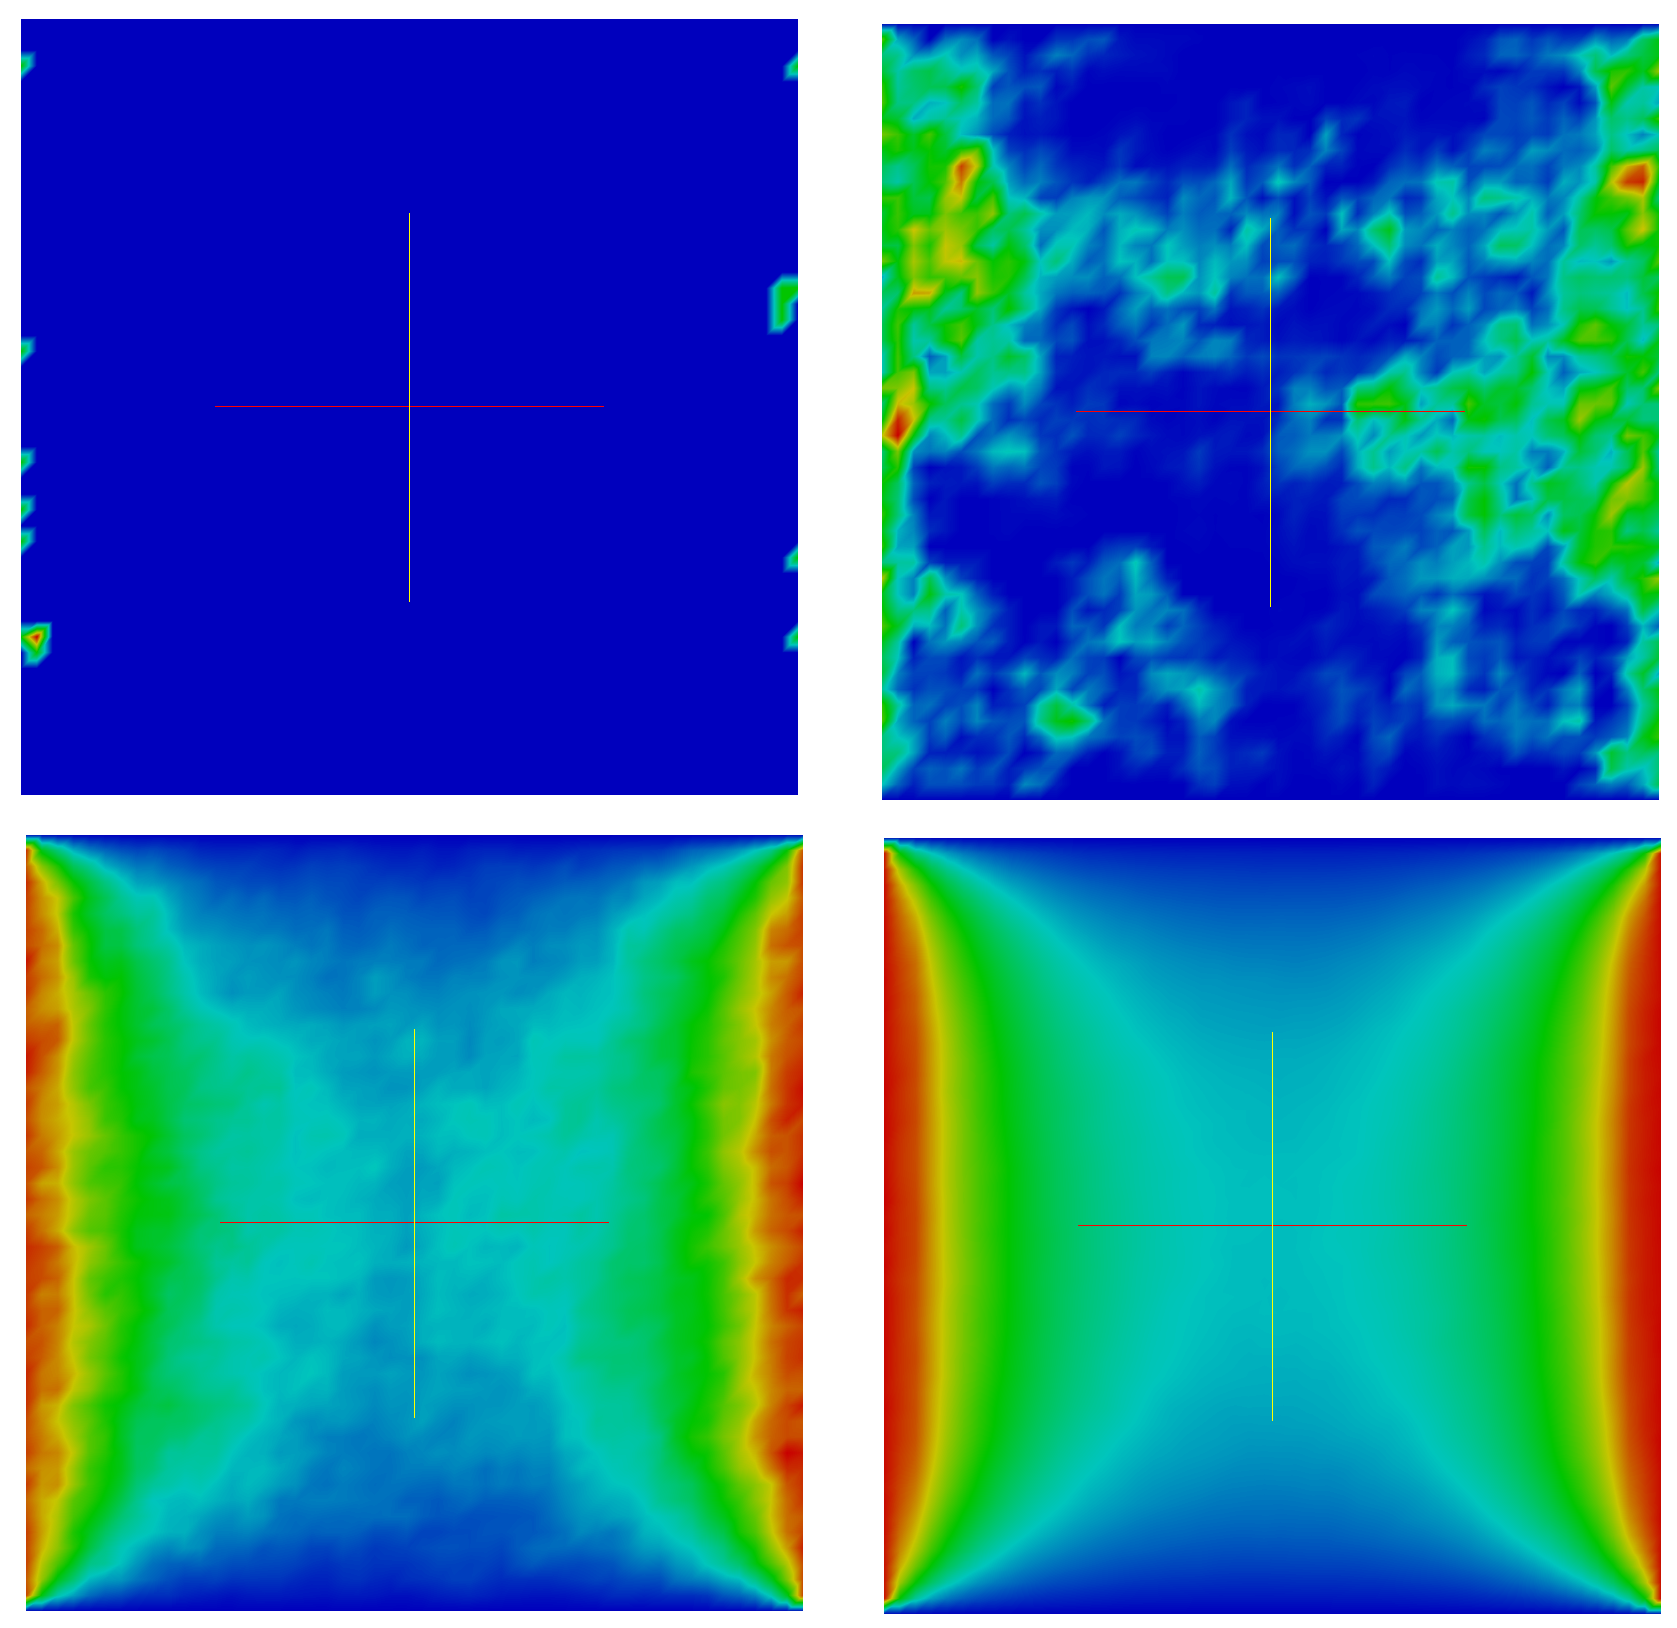
\includegraphics[width=5in]{chapters/mc_background/adjoint_evolution.png}
  \end{center}
  \caption{\textbf{Adjoint Monte Carlo solution to the heat equation
      with varying numbers of histories.} \textit{Top left: 10
      histories per state. Top right: 1,000 histories per
      state. Bottom left: 100,000 histories per state. Bottom right:
      10,000,000 histories per state.}}
  \label{fig:adjoint_evolution}
\end{figure}
As the number of histories used per state is increased, the
statistical variance of the solutions is decreased as more tallies are
made. At 10,000,000 histories per state, enough tallies have been made
to generate a reasonable estimate for the structure of the
solution. The visual difference between
Figures~\ref{fig:direct_evolution} and \ref{fig:adjoint_evolution} is
precisely that determined by their mathematics. As the adjoint
solution evolves with the addition of histories, more histories
emanate from the source with more penetrating the domain and making
contributions to those tallies. As the direct method evolves, the
solution simply comes into focus as histories are emanated from each
state in the system and contribute only to the solution in that state
regardless of their path.

%%---------------------------------------------------------------------------%%
\section{Sequential Monte Carlo}
\label{sec:sequential_mc}
The direct and adjoint Neumann-Ulam methods described are limited by a
convergence rate of $1/\sqrt{N}$ by the Central Limit Theorem where
$N$ is the number of random walk permutations. In 1962, Halton
presented a residual Monte Carlo method that moves towards exponential
convergence rates \citep{halton_sequential_1962} and further refined
his work some years later \citep{halton_sequential_1994}. Applications
of his work by the transport community have confirmed convergence
rates on the order of of $exp(-N)$ \citep{evans_residual_2003}. In
much the same way as projection methods, Halton's method, sequential
Monte Carlo, utilizes the adjoint Monte Carlo solver as a means of
directly reducing the residual vector. He proposed the following
iterative scheme as a solution to Eq~(\ref{eq:linear_problem})\:
\begin{subequations}
  \begin{gather}
    \ve{r}^k = \ve{b} - \ve{A}\ve{x}^k\:,\\  
    \ve{A}\boldsymbol{\delta}^{k} = \ve{r}^{k}\:,\\
    \ve{x}^{k+1} = \ve{x}^k + \boldsymbol{\delta}^{k}\:,
  \end{gather}
  \label{eq:sequential_monte_carlo}
\end{subequations}
where the correction $\boldsymbol{\delta}$ is computed by the adjoint
Monte Carlo method. The merits of Halton's approach are immediately
visible in that we have now broken the binding of the convergence rate
to the Central Limit Theorem. Here, the Monte Carlo solver is used to
produce a correction from the residual, analogous to using the
residual to extract a correction from the search subspace in a
projection method. By doing this, the Monte Carlo error is bound in
the correction used to update the solution and therefore does not
explicitly manifest itself in the overall convergence of the
solution. The downside of such a method is that if the solution guess
is poor, then many iterations are required in order to reach
exponential converge as the Monte Carlo error (and therefore the
Central Limit Theorem) does dominate in this situation. Therefore, if
a good initial guess is not available, Halton's method is still
characterized by poor performance.

%%---------------------------------------------------------------------------%%
\section{Monte Carlo Synthetic-Acceleration}
\label{sec:mcsa}
Using the ideas of Halton, Evans and Mosher recently developed a Monte
Carlo solution method that was not prohibited severely by the quality
of the initial guess for the system \citep{evans_monte_2009} and later
applied it more rigorously as a solution mechanism for the radiation
diffusion equation \citep{evans_monte_2012}. With their new methods,
they achieved identical numerical results as and marginally better
performance than conventional Krylov solvers. Their approach was
instead to use residual Monte Carlo as a synthetic acceleration for a
stationary method. To derive this method, we begin by splitting the
operator in Eq~(\ref{eq:linear_problem})
\begin{equation}
  \ve{x} = (\ve{I} - \ve{A})\ve{x} + \ve{b}\:.
  \label{eq:linear_split}
\end{equation}
With this we can then define the stationary method
\textit{Richardson's iteration} as:
\begin{equation}
  \ve{x}^{k+1} = (\ve{I} - \ve{A})\ve{x}^k + \ve{b}\:,
  \label{eq:richardsons_iteration}
\end{equation}
which will converge if $\rho(\ve{I} - \ve{A}) < 1$. We then define the
solution error at the $k^{th}$ iterate relative to the true solution:
\begin{equation}
  \delta \ve{x}^k = \ve{x} - \ve{x}^k\:.
  \label{eq:mcsa_error}
\end{equation}
Subtracting Eq~(\ref{eq:richardsons_iteration}) from
Eq~(\ref{eq:linear_split}) we get:
\begin{equation}
  \delta \ve{x}^{k+1} = (\ve{I} - \ve{A})\delta \ve{x}^k\:.
  \label{eq:mcsa_setup_1}
\end{equation}
Subtracting from this $(\ve{I} - \ve{A})\delta \ve{x}^{k+1}$ yields:
\begin{equation}
  \begin{split}
    \ve{A}\delta \ve{x}^{k+1} &= (\ve{I} -
    \ve{A})(\ve{x}^{k+1}-\ve{x}^{k}) \\ &= \ve{r}^{k+1}\:.
    \label{eq:mcsa_setup_2}
  \end{split}
\end{equation}
Using this, we define the following scheme that will converge in one
iteration if $\ve{A}$ is inverted exactly.
\begin{subequations}
  \begin{gather}
    \ve{x}^{k+1} = (\ve{I} - \ve{A})\ve{x}^k + \ve{b}\:,\\
    \ve{A} \delta \ve{x}^{k+1} = \ve{r}^{k+1}\:,\\
    \ve{x} = \ve{x}^{k+1} + \delta \ve{x}^{k+1}\:.
  \end{gather}
  \label{eq:mcsa_setup_3}
\end{subequations}
However, $\ve{A}$ is only approximately inverted by our numerical
methods and therefore we instead pose an iterative scheme in which the
Monte Carlo solvers are used to invert the operator. The
\textit{Fixed-Point Monte Carlo Synthetic-Acceleration} (MCSA) method
is defined as:
\begin{subequations}
  \begin{gather}
    \ve{x}^{k+1/2} = \ve{x}^k + \ve{r}^k\:,\\
    \ve{r}^{k+1/2} = \ve{b} - \ve{A}\ve{x}^{k+1/2}\:,\\
    \ve{A}\delta\ve{x}^{k+1/2} = \ve{r}^{k+1/2}\:,\\
    \ve{x}^{k+1} = \ve{x}^{k+1/2} + \delta \ve{x}^{k+1/2}\:,
  \end{gather}
  \label{eq:mcsa}
\end{subequations}
where the adjoint Monte Carlo method is used to generate the solution
correction from the residual. Using Monte Carlo in this way achieves
the same effect as Halton's method, decoupling its convergence rate
from the overall convergence rate of the method. Here, the approximate
Monte Carlo solution is not driven to a particular convergence as it
merely supplies a correction for the initial guess generated by
Richardson's iteration. Rather, only a set number of histories are
required using the adjoint method to generate the correction.

In addition to the Monte Carlo solver parameters dictating the number
of histories and weight cutoff, the outer MCSA iterations also have
the following stopping criteria:
\begin{equation}
  ||\ve{r}||_\infty < \epsilon \ ||\ve{b}||_\infty\:,
  \label{eq:mcsa_stopping_criteria}
\end{equation}
where $\epsilon$ is a user-defined parameter. We therefore have 3
parameters to tune in an MCSA implementation: the number of Monte
Carlo histories computed in the adjoint solve during each MCSA
iteration, the weight cutoff for those histories, and the total MCSA
convergence tolerance as specified by $\epsilon$.

\subsection{Preconditioning MCSA}
\label{sec:stochastic_preconditioning}
In most cases, at least a minimal amount of \textit{preconditioning}
of the linear system will be required in order to use the class of
stochastic methods described. Although these methods have no symmetry
requirements for convergence, they do require that the spectral radius
of the iteration matrix be less than one. To achieve this for
diagonally dominant matrices, a point Jacobi preconditioner, a form of left
preconditioning, is used such that the preconditioning matrix $\ve{M}$
is:
\begin{equation}
  \ve{M} = diag(\ve{A})\:,
  \label{eq:jacobi_preconditioner}
\end{equation}
such that its application means we are instead solving the following
linear system:
\begin{equation}
  \ve{M}^{-1}\ve{A}\ve{x} = \ve{M}^{-1}\ve{b}\:.
  \label{eq:jacobi_precond_linear_problem}
\end{equation}
Next, we can apply MCSA to solve
Eq~(\ref{eq:jacobi_precond_linear_problem}): 
\begin{subequations}
  \begin{gather}
    \ve{x}^{k+1/2} = \ve{x}^k +
    \ve{M}^{-1}\ve{r}^k\:,\\ \ve{r}^{k+1/2} =
    \ve{b}-\ve{A}\ve{x}^{k+1/2}\:,\\ \ve{M}^{-1}\ve{A}\delta\ve{x}^{k+1/2}
    = \ve{M}^{-1}\ve{r}^{k+1/2}\:,\\ \ve{x}^{k+1} = \ve{x}^{k+1/2} +
    \delta \ve{x}^{k+1/2}\:.
    \label{eq:jacobi_preconditioned_mcsa}
  \end{gather}
\end{subequations}
Choosing point Jacobi preconditioning with MCSA is advantageous for
several reasons. First, $\rho(\ve{I} - \ve{M}^{-1}\ve{A}) < 1$ is true
for all $\ve{A}$ that is diagonally dominant and is easy to formulate
because the inversion of $\ve{M}$ is trivial. Second, because the
adjoint Monte Carlo method used within MCSA to compute the correction
operates on a linear problem with the preconditioned operator, then
$\ve{H}$ in the adjoint solver will have a zero term in each of its
diagonal elements, thereby eliminating all in-state transitions during
the random walk sequence. Because of this, point Jacobi
preconditioning should almost always be performed, regardless of any
other preconditioning that is applied to the system.

%%---------------------------------------------------------------------------%%
\section{Monte Carlo Method Selection}
The MCSA method defined in Eq.~(\ref{eq:mcsa}) uses the adjoint method
to estimate the error in residual Monte Carlo solve instead of the
direct method outlined in \S~\ref{sec:direct_mc}. To demonstrate
the effectiveness of the adjoint method over the direct method within
the context of MCSA, we choose the 2D time-dependent Poisson equation
as a simple model problem:
\begin{equation}
  \frac{\partial \ve{u}}{\partial t} = \nabla^2 \ve{u}\:.
  \label{eq:poisson_equation}
\end{equation}
For all comparisons, a single time step is computed with backwards Euler time
integration. The Laplacian is differenced on a square Cartesian grid with a
second-order five-point stencil,
\begin{equation}
  \nabla^2_5 = \frac{1}{\Delta^2}[u_{i-1,j} + u_{i+1,j} + u_{i,j-1} +
    u_{i,j+1} - 4 u_{i,j}]\:,
  \label{eq:five_point_stencil}
\end{equation}
and a fourth-order nine-point stencil,
\begin{multline}
  \nabla^2_9 = \frac{1}{6\Delta^2}[4 u_{i-1,j} + 4 u_{i+1,j} + 4
    u_{i,j-1} + 4 u_{i,j+1} + u_{i-1,j-1}\\ + u_{i-1,j+1} +
    u_{i+1,j-1} + u_{i+1,j+1} - 20 u_{i,j}]\:,
  \label{eq:nine_point_stencil}
\end{multline}
both assuming a grid size of $\Delta$ in both the $i$ and $j$ directions. For
a single time step solution, we then have the following sparse linear system
to be solved with the MCSA method:
\begin{equation}
  \ve{A} \ve{u}^{n+1} = \ve{u}^n\:.
  \label{eq:poisson_eq_lin_sys}
\end{equation}
Both the stencils will be used to vary the size and density of the sparse
linear system in Eq.~(\ref{eq:poisson_eq_lin_sys}).

A timing and convergence study is used to demonstrate the
effectiveness of the adjoint method as compared to the direct
method. To assess both the CPU time and number of iterations required
to converge to a solution, a problem of constant $\Delta$ was used
with varying values of grid size, fixing the spectral radius of the
system at a constant value for each variation. Both the five-point and
nine-point stencils were used with both the direct and adjoint
solvers. For each case, $N \times N$ total random walk permutations
were computed per MCSA iteration where $N \times N$ is the number of
discrete grid points in the system. Solver parameters were set to a
weight cutoff of \sn{1}{-4} for the stochastic linear solver and a
convergence tolerance of \sn{1}{-8} for the MCSA iterative solver.
Figure~\ref{fig:poisson_cpu_time} gives the CPU time needed for each
case to converge in seconds and Figure~\ref{fig:poisson_iterations}
gives the number of iterations needed for each case to converge to the
specified tolerance as a function of the problem size. All
computations presented in this section and
\S~\ref{subsec:sequential_comparison} were completed on a 3.0 GHz
Intel Core 2 Quad Q9650 CPU machine with 16 GB 1067 MHz DDR3 memory.
\begin{figure}[ht!]
  \centering
  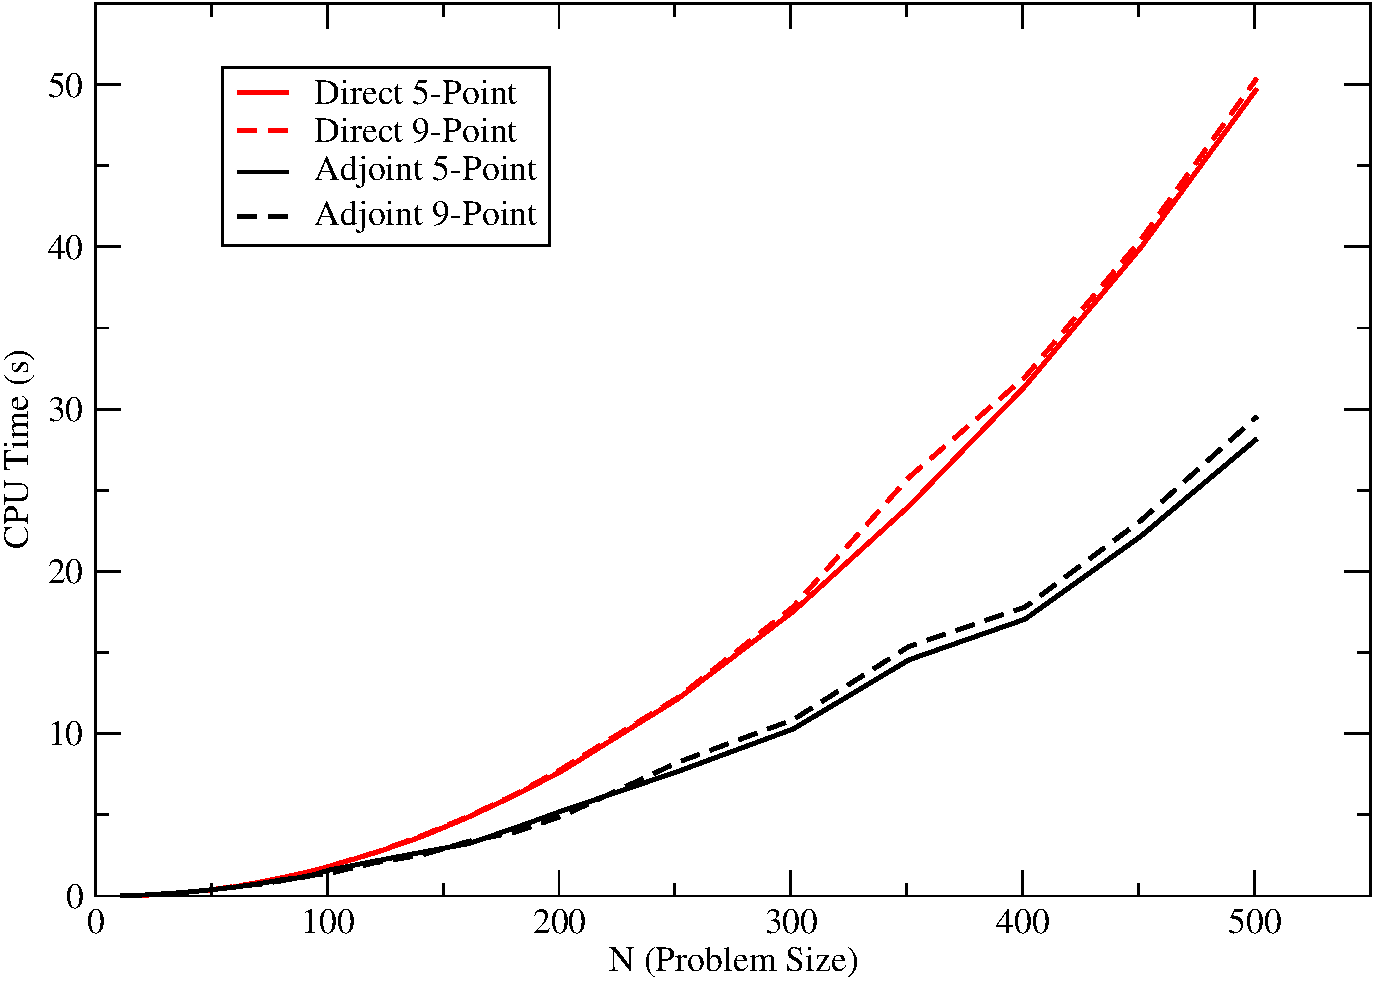
\includegraphics[width=5in,clip]{chapters/mc_background/dir_adj_cpu.pdf}
  \caption{\textbf{CPU Time (s) to converge vs. Problem Size ($N$ for
      an $N \times N$ square mesh).} \textit{Both the adjoint and
      direct solvers are used with the five point and nine point
      stencils. A CPU time speedup is noted with the adjoint method
      due to the higher density of random walk events in regions with
      a large residual.}}
  \label{fig:poisson_cpu_time}
\end{figure}

\begin{figure}[ht!]
  \centering
  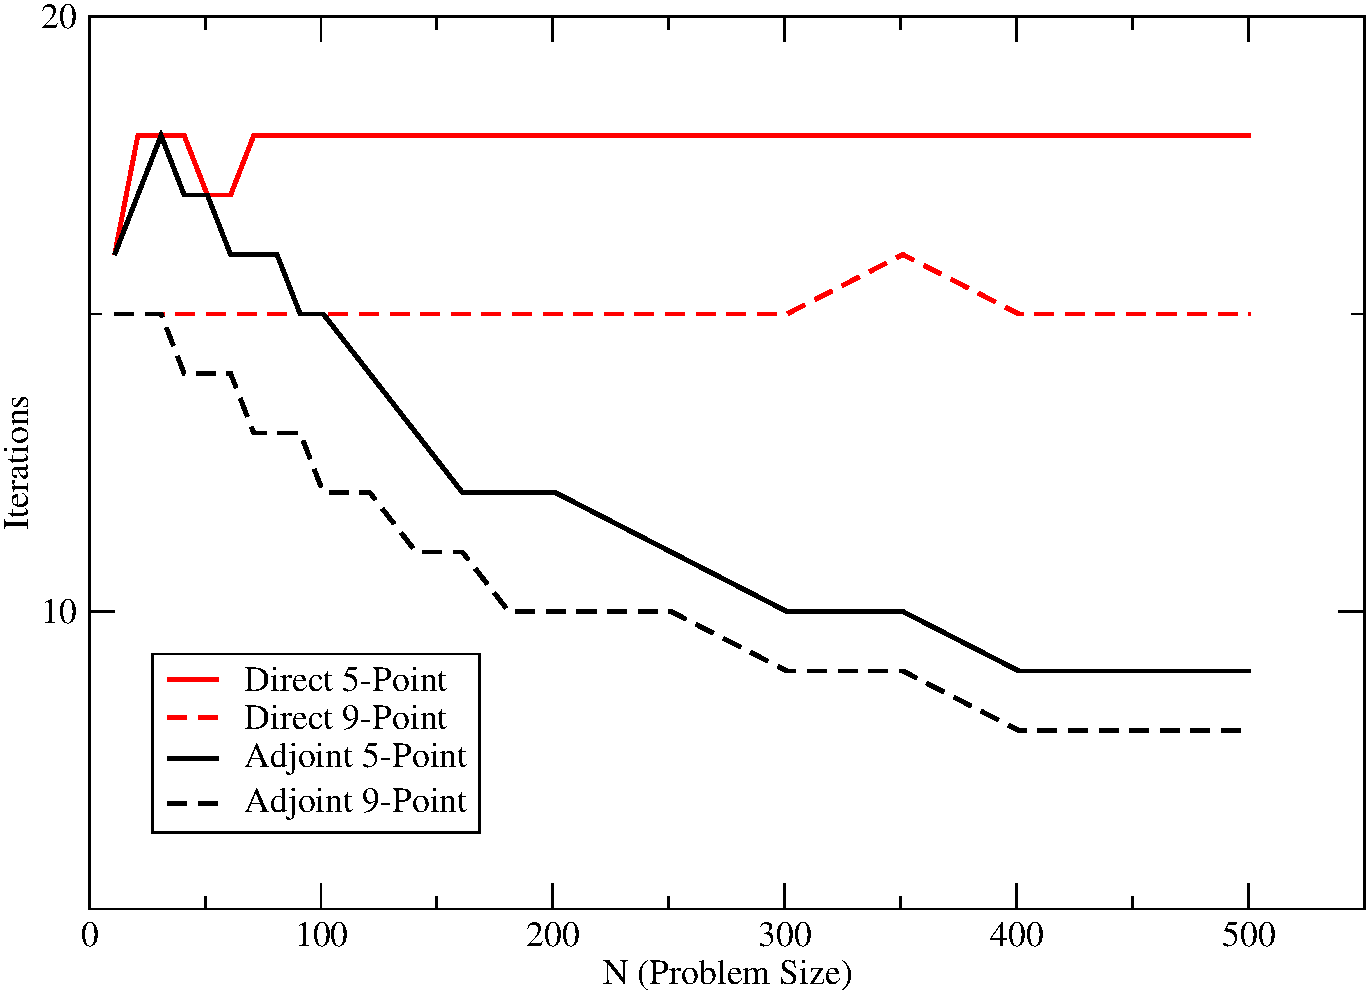
\includegraphics[width=5in,clip]{chapters/mc_background/dir_adj_iterations.pdf}
  \caption{\textbf{Iterations to converge vs. Problem Size ($N$ for an
      $N \times N$ square mesh).} \textit{Both the adjoint and direct
      solvers are used with the five-point and nine-point stencils.}}
  \label{fig:poisson_iterations}
\end{figure}

We see clearly in Figure~\ref{fig:poisson_cpu_time} that the using the
adjoint solver with MCSA results in a speedup over the direct solver
while the number of iterations required to converge is also reduced as
shown in Figure~\ref{fig:poisson_iterations}. We expect this for several
reasons. First, with an equivalent number of histories specified for
both solvers per MCSA iteration and a system of size $N \times N$, the
direct solver will compute a single random walk for each state in the
system per iteration to acquire a solution in that state, regardless
of the size of the residual in that state. This is necessary in the
direct method to ensure a contribution from each state as the random
walk sequence will only contribute to the starting state. For the
adjoint method, a total of $N \times N$ random walk events will have
their starting state determined by sampling the residual
vector. Because the random walk sequence contributes to the state in
which it currently resides, sampling the residual vector as the Monte
Carlo source gives a higher density of random walk events in regions
with a high residual, thus giving a more accurate correction in that
region due to reduced statistical error. From an iteration
perspective, Figure~\ref{fig:poisson_iterations} shows that using the
direct method yields a roughly unchanging number of iterations
required to converge as the problem size increases. Again, if we
desire a correction value for all states in the problem, then we must
start a random walk in each state in the system which does not reduce
the number of iterations need as the problem size grows. Conversely,
as the problem size grows in the adjoint method, the additional
stochastic histories that will be computed are concentrated in regions
with a large residual, further reducing the stochastic error in the
correction in those regions and subsequently reducing the required
number of iterations to converge.

As an additional comparison, the convergence behavior of MCSA can be
analyzed using both the adjoint and direct solvers to detect any
performance benefits. To assess the convergence properties of MCSA
using each solver and stencil, the infinity norm of the residual
computed in Eq.~(\ref{eq:mcsa}) was collected at each iteration for a
fixed problem size of $N=500$. Figure~\ref{fig:poisson_convergence}
gives the results of these computations. First, it is worthy to note
on the semilog plot that we are indeed achieving the expected
exponential convergence from MCSA with both Monte Carlo
solvers. Second, we note that using the adjoint method with the same
number of stochastic histores per MCSA iteration gives a faster rate
of converge for the same reasons as above. We also note here that
fewer iterations are required for convergence when the 9-point stencil
is used to discretize the Laplacian operator (although at no gain in
speed as given by the results in
Figure~\ref{fig:poisson_cpu_time}). This is due to the fact that the
smaller discretization error directly corresponds to a more well
defined residual source generated by the Richardson extrapolation for
the Monte Carlo calculation. In addition, the better defined source is
transported through a domain described more accurately by the 9-point
stencil, thus yielding a more accuracte correction vector from the
Monte Carlo calculation.

\begin{figure}[ht!]
  \centering
  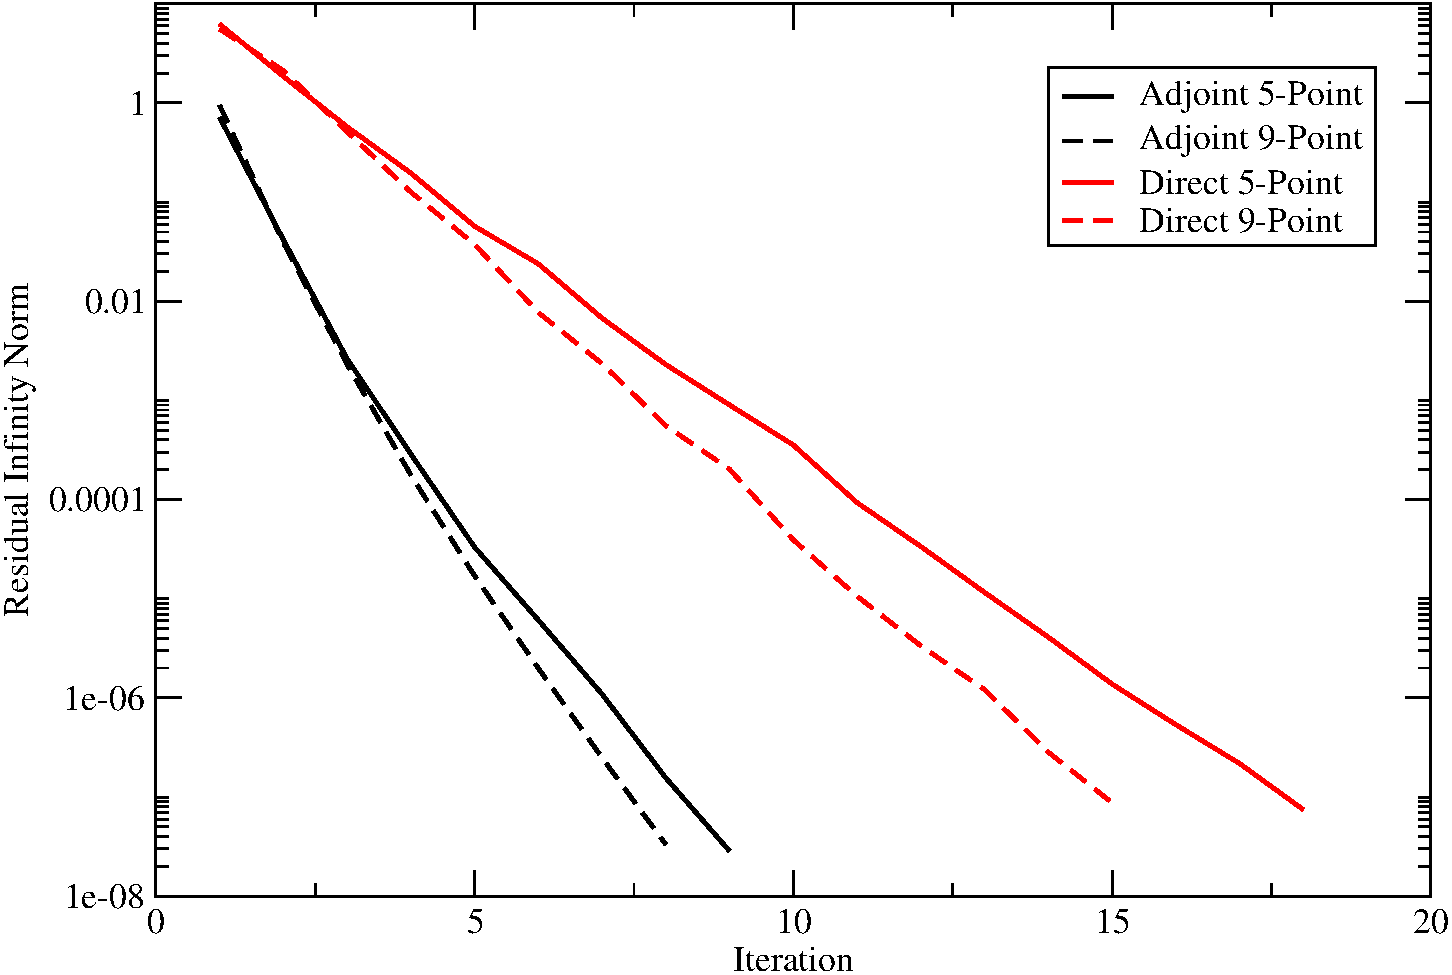
\includegraphics[width=5in,clip]{chapters/mc_background/dir_adj_conv.pdf}
  \caption{\textbf{Infinity norm of the solution residual
      vs. iteration number for a problem of size $N=500$.}
    \textit{Both the adjoint and direct solvers are used with the five
      point and nine point stencils. A higher rate of convergence is
      observed for MCSA using the adjoint Monte Carlo solver as
      compared to the direct method when both solvers compute the same
      number of random walks per iteration.}}
  \label{fig:poisson_convergence}
\end{figure}

%%---------------------------------------------------------------------------%%
\section{MCSA Comparison to Sequential Monte Carlo}
\label{subsec:sequential_comparison}
To further motivate using Monte Carlo Synthetic Acceleration, we
compare its performance to Halton's Sequential Monte Carlo method on
which our previous work in this area was based. For this comparison,
we use the same transient Poisson problem as described in the previous
section and choose only the 5-point stencil to discretize the
Laplacian operator as the previous results yielded little qualitative
difference between the discretizations. Both MCSA and Halton's method
are used with the adjoint Monte Carlo solver. In order to complete the
same study as in the previous section, the number of histories
computed by the Monte Carlo solver at each iteration had to be doubled
to $2 \times N \times N$ in order to ensure convergence in Sequential
Monte Carlo Method. Figure~\ref{fig:seq_cpu_time} gives the CPU time
results for this comparison as a function of problem size while
Figure~\ref{fig:seq_iterations} gives the number of iterations to
converge as a function of problem size. In both cases, using the Monte
Carlo solver as a synthetic acceleration rather than in a pure
residual Monte Carlo scheme resulted in a reduction in both CPU time
and iterations required to converge. The additional Richardson
extrapolation between each Monte Carlo solve in the MCSA method gives
a better converged residual source to use with the Monte Carlo
calculation while the Sequential method requires more iterations to
achieve the same level of convergence in the residual.

\begin{figure}[ht!]
  \centering
  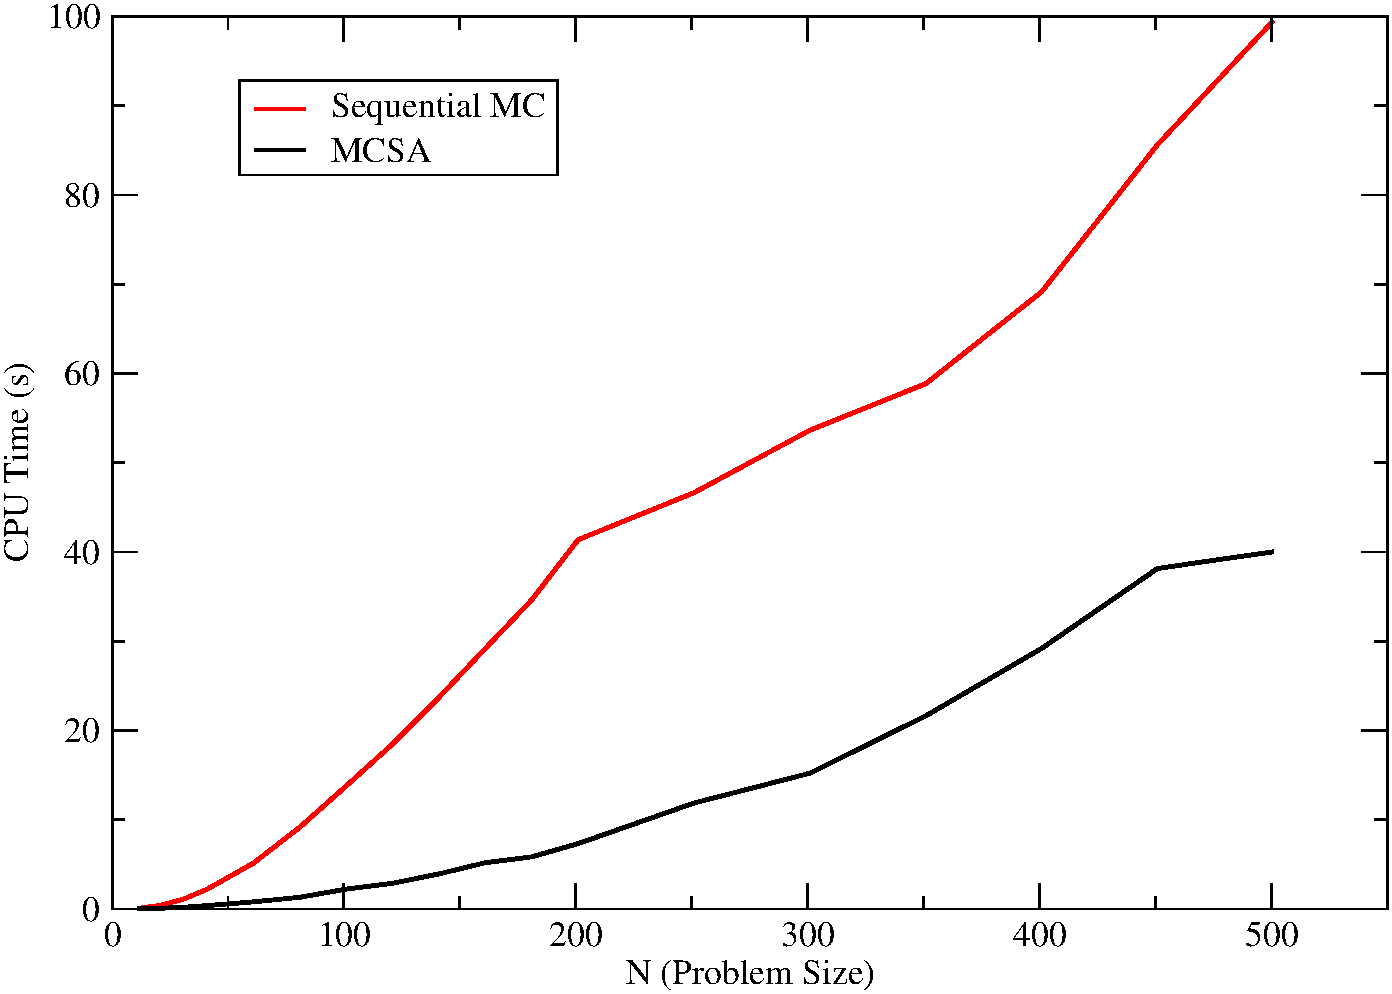
\includegraphics[width=5in,clip]{chapters/mc_background/seq_cpu.pdf}
  \caption{\textbf{CPU Time (s) to converge vs. Problem Size ($N$ for
      an $N \times N$ square mesh).} \textit{oth the Sequential Monte
      Carlo and MCSA solvers are used with the five point stencils and
      the adjoint Monte Carlo solver. The number of random walks was
      twice the number of discrete states in the system in order to
      ensure convergence in the Sequential Monte Carlo method.}}
  \label{fig:seq_cpu_time}
\end{figure}

\begin{figure}[ht!]
  \centering
  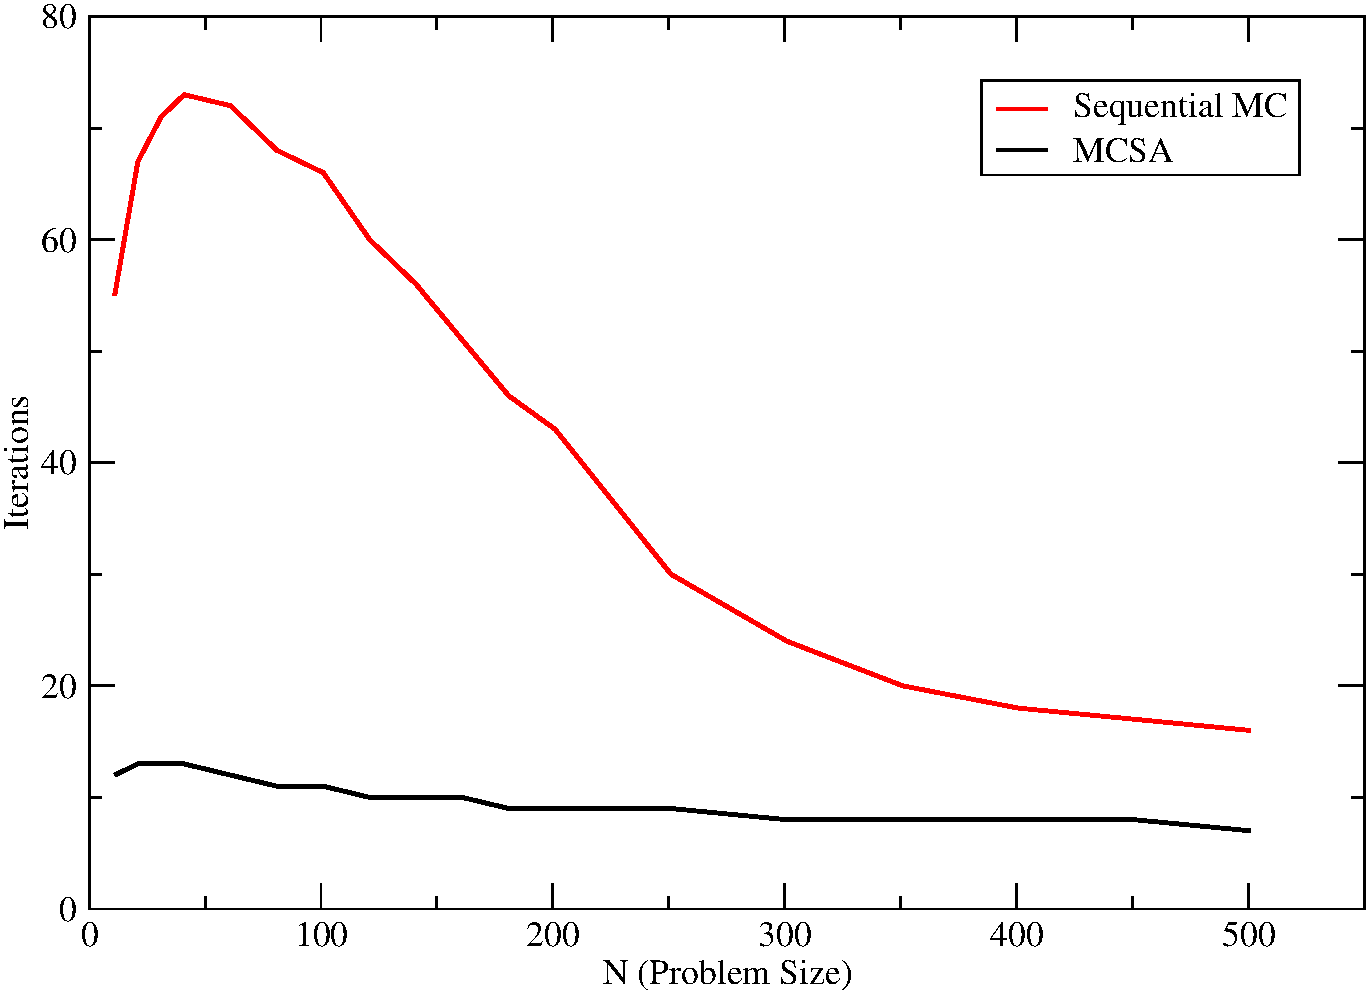
\includegraphics[width=5in,clip]{chapters/mc_background/seq_iterations.pdf}
  \caption{\textbf{Iterations to converge vs. Problem Size ($N$ for an
      $N \times N$ square mesh).} \textit{Both the Sequential Monte
      Carlo and MCSA solvers are used with the five point stencils and
      the adjoint Monte Carlo solver.}}
  \label{fig:seq_iterations}
\end{figure}

The benefits of using a synthetic acceleration scheme are also noted
when the infinity norm of the residual computed at each iteration for
both methods was collected at each iteration for a fixed problem sizes
of $N=100$ and $N=500$ as shown in figures Figure~\ref{fig:seq_100}
and \ref{fig:seq_500} respectively. In both cases, the Sequential
method is subject to two regimes of exponential convergence with the
later regime converging the slowest while the MCSA method exhibits a
single rate of exponential convergence observed to be much higher than
that computed by Halton's method. Even with the doubling of the number
of stochastic histories computed per time step in order to ensure
convergence for the Sequential method, we still see robustness issues
with a non-monotonically decreasing residual observed for the $N=100$
case. In both cases the MCSA solver is observed to be robust with a
monotonically decreasing residual.

\begin{figure}[ht!]
  \centering
  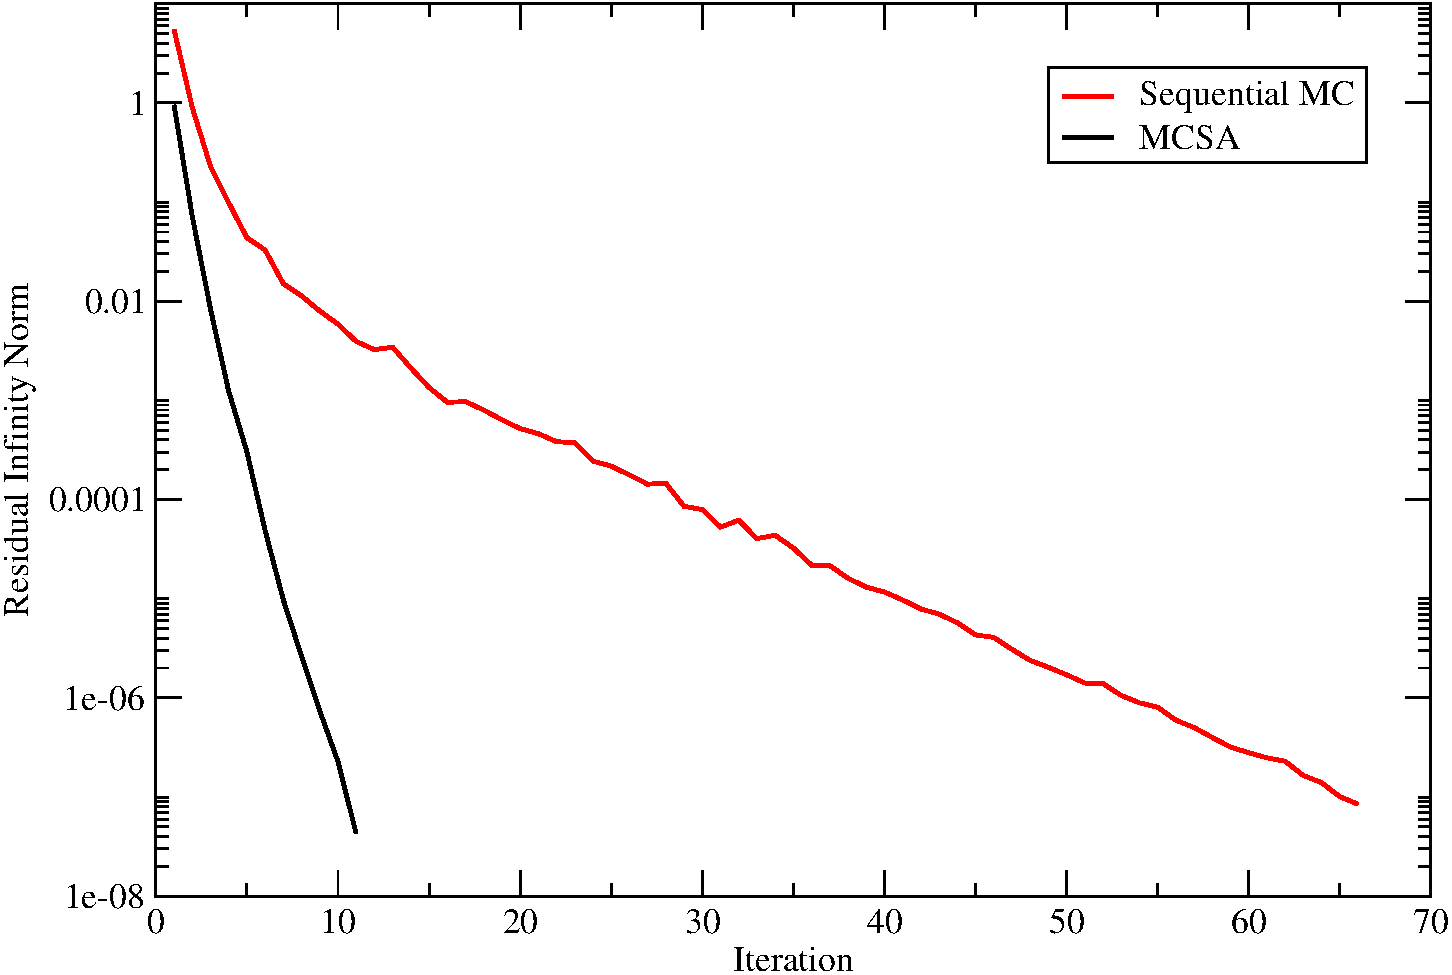
\includegraphics[width=5in,clip]{chapters/mc_background/seq_conv_100.pdf}
  \caption{\textbf{Infinity norm of the solution residual
      vs. iteration number for a problem of size $N=100$.}
    \textit{Both the Sequential Monte Carlo and MCSA solvers are used
      with the five point stencils and the adjoint Monte Carlo
      solver.}}
  \label{fig:seq_100}
\end{figure}

\begin{figure}[ht!]
  \centering
  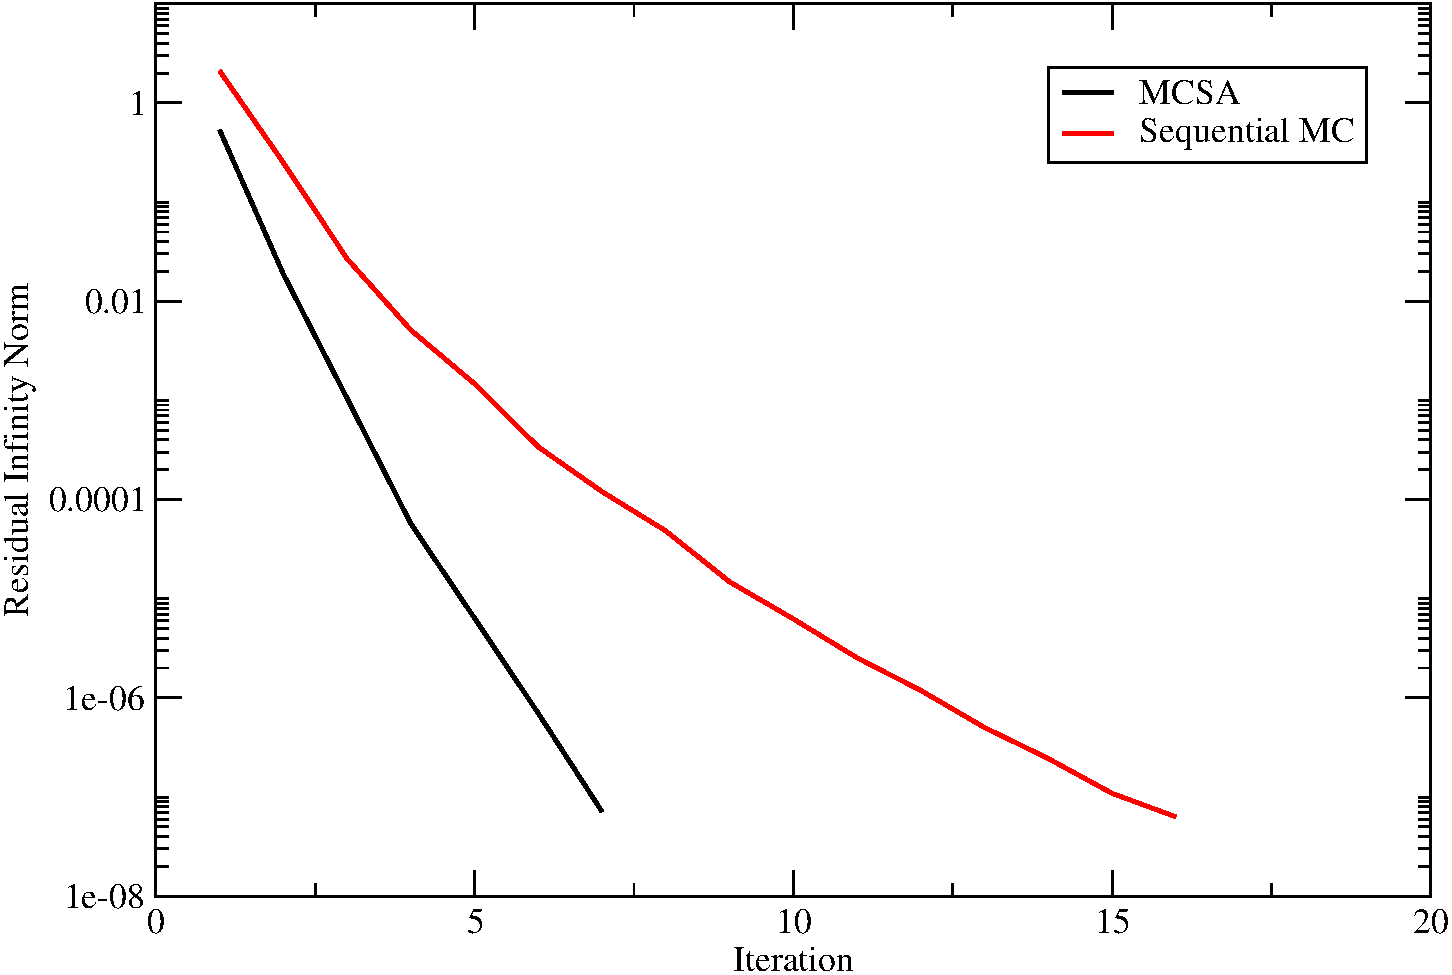
\includegraphics[width=5in,clip]{chapters/mc_background/seq_conv_500.pdf}
  \caption{\textbf{Infinity norm of the solution residual
      vs. iteration number for a problem of size $N=500$.}
    \textit{Both the Sequential Monte Carlo and MCSA solvers are used
      with the five point stencils and the adjoint Monte Carlo
      solver.}}
  \label{fig:seq_500}
\end{figure}
